\documentclass{ximera}

\begin{document}
	\author{Stitz-Zeager}
	\xmtitle{Exercises for Rational Graphs}{}

\mfpicnumber{1} \opengraphsfile{ExercisesforRationalGraphs} % mfpic settings added 

Suppose $r$ is a rational function.  You can graph the function $r$ using the following six-step procedure:

\begin{enumerate}

\item  Find the domain of $r$.

\item  Reduce $r(x)$ to lowest terms, if applicable.\footnote{This helps us determine limits for the next step.}

\item  Determine the location of any vertical asymptotes or holes in the graph, if they exist. 

\item  Find the axis intercepts, if they exist.

\item  Analyze the end behavior of $r$.  Find the horizontal or slant asymptote, if one exists.

\item  Use a sign diagram and plot additional points, as needed, to sketch the graph.\footnote{It doesn't hurt to check for symmetry at this point, if convenient.}

\end{enumerate}

\begin{problem}\label{sixstepfirst}
Use the six-step procedure
to graph the rational function.  Be sure to draw any asymptotes as dashed lines.

$f(x) = \dfrac{4}{x + 2}$

\begin{solution}
\[
\graph[xmin=-7, xmax=5, ymin=-5, ymax=5,panel]{f(x)=\frac{4}{x+2}}
\]
\end{solution}
\end{problem}

\begin{problem}
Use the six-step procedure
to graph the rational function.  Be sure to draw any asymptotes as dashed lines.

$f(x) = 5x(6-2x)^{-1}$ 
\end{problem}  

\begin{problem}
Use the six-step procedure
to graph the rational function.  Be sure to draw any asymptotes as dashed lines.

$g(t) = t^{-2}$
\end{problem} 

\begin{problem}
Use the six-step procedure
to graph the rational function.  Be sure to draw any asymptotes as dashed lines.

$g(t) = \dfrac{1}{t^{2} + t - 12}$
\end{problem}

\begin{problem}
Use the six-step procedure
to graph the rational function.  Be sure to draw any asymptotes as dashed lines.

$r(z) = \dfrac{2z - 1}{-2z^{2} - 5z + 3}$

\begin{solution}
\[
\graph[xmin=-7, xmax=5, ymin=-5, ymax=5,panel]{r(z) = \dfrac{2z - 1}{-2z^{2} - 5z + 3}}
\]
\end{solution}
\end{problem} 

\begin{problem}
Use the six-step procedure
to graph the rational function.  Be sure to draw any asymptotes as dashed lines.

$r(z) = \dfrac{z}{z^{2} + z - 12}$
\end{problem}  

\begin{problem}
Use the six-step procedure
to graph the rational function.  Be sure to draw any asymptotes as dashed lines.

$f(x) = 4x(x^2+4)^{-1}$
\end{problem} 

\begin{problem}
Use the six-step procedure
to graph the rational function.  Be sure to draw any asymptotes as dashed lines.

$f(x) = 4x(x^2-4)^{-1}$
\end{problem} 

\begin{problem}
Use the six-step procedure
to graph the rational function.  Be sure to draw any asymptotes as dashed lines.

$g(t) = \dfrac{t^2-t-12}{t^2+t-6}$

\begin{solution}
\[
\graph[xmin=-7, xmax=5, ymin=-5, ymax=5,panel]{g(t) = \dfrac{t^2-t-12}{t^2+t-6}}
\]
\end{solution}
\end{problem} 

\begin{problem}
Use the six-step procedure
to graph the rational function.  Be sure to draw any asymptotes as dashed lines.

$g(t) = 3- \dfrac{5t-25}{t^2-9}$
\end{problem} 

\begin{problem}
Use the six-step procedure
to graph the rational function.  Be sure to draw any asymptotes as dashed lines.

$r(z) = \dfrac{z^2-z-6}{z+1}$
\end{problem}  

\begin{problem}
Use the six-step procedure
to graph the rational function.  Be sure to draw any asymptotes as dashed lines.

$r(z) =-z-2+\dfrac{6}{3-z}$
\end{problem} 

\begin{problem}
Use the six-step procedure
to graph the rational function.  Be sure to draw any asymptotes as dashed lines.

$f(x) = \dfrac{x^3+2x^2+x}{x^2-x-2}$

\begin{solution}
\[
\graph[xmin=-7, xmax=5, ymin=-5, ymax=5,panel]{f(x) = \dfrac{x^3+2x^2+x}{x^2-x-2}}
\]
\end{solution}
\end{problem}  

\begin{problem}
Use the six-step procedure
to graph the rational function.  Be sure to draw any asymptotes as dashed lines.

$f(x) = \dfrac{5x}{9-x^2} - x$
\end{problem}   

\begin{problem}
Use the six-step procedure
to graph the rational function.  Be sure to draw any asymptotes as dashed lines.

$g(t) =\dfrac{1}{2}t-1 + \dfrac{t+1}{t^2+1}$
\end{problem} 

\begin{problem}\label{sixsteplast}
Use the six-step procedure
to graph the rational function.  Be sure to draw any asymptotes as dashed lines.\footnote{Once you've done the six-step procedure, use a graphing utility to graph this function on the window $[0, 12] \times [0, 0.25]$ \ldots}

$g(t) = \dfrac{t^{2} - 2t + 1}{t^{3} + t^{2} - 2t}$ 
\end{problem} 

\begin{problem}\label{rationalfromgraphfirst}
Find a possible formula for the function whose graph is given.
$y = f(x)$

\begin{tikzpicture}
  \begin{axis}[
    axis lines=middle,
    xmin=-2, xmax=6,
    ymin=-4, ymax=4,
    xtick={-1,0,1,2,3,4,5},
    xticklabels={$-1$,$0$,$1$,$2$,$3$,$4$,$5$},
    ytick={-3,-2,-1,1,2,3},
    yticklabels={$-3$,$-2$,$-1$,$1$,$2$,$3$},
    axis line style={->},
    width=11cm, height=8cm,
    clip=false
  ]
    % Axis labels
    \node at (axis cs:6,-0.5) {\scriptsize $x$};
    \node at (axis cs:0.5,4) {\scriptsize $y$};

    % Vertical asymptote
    \addplot[dashed] coordinates {(2,-4) (2,4)};

    % Function pieces (avoiding vertical asymptote at x=2)
    \addplot[domain=-2:1.75, samples=200, thick, ->] {1/(x-2)};
    \addplot[domain=2.25:6, samples=200, thick, ->] {1/(x-2)};

    % Points
    \addplot[only marks, mark=*] coordinates {(1,-1) (3,1)};

    % Point labels
    \node at (axis cs:3.75,1.25) {\scriptsize $(3,1)$};
    \node at (axis cs:0.5,-1.5) {\scriptsize $(1,-1)$};

    % Caption below
    \node[below] at (rel axis cs:0.5,0) 
      {\scriptsize Vertical asymptote: $x=2$};
  \end{axis}
\end{tikzpicture}

\begin{solution}
$f(x) = \dfrac{1}{x - 2}$
\end{solution}
\end{problem}

\begin{problem}
Find a possible formula for the function whose graph is given.
$y = F(x)$

\begin{tikzpicture}
  \begin{axis}[
    axis lines=middle,
    xmin=-2, xmax=6,
    ymin=-4, ymax=4,
    xtick={-1,0,1,2,3,4,5},
    xticklabels={$-1$,$0$,$1$,$2$,$3$,$4$,$5$},
    ytick={-3,-2,-1,1,2,3},
    yticklabels={$-3$,$-2$,$-1$,$1$,$2$,$3$},
    axis line style={->},
    width=11cm, height=8cm,
    clip=false
  ]
    % Axis labels
    \node at (axis cs:6,-0.5) {\scriptsize $x$};
    \node at (axis cs:0.5,4) {\scriptsize $y$};

    % Vertical asymptote
    \addplot[dashed] coordinates {(2,-4) (2,4)};

    % Function pieces (avoiding asymptote at x=2)
    \addplot[domain=-2:1.75, samples=200, thick, ->] {1/(x-2)};
    \addplot[domain=2.25:6, samples=200, thick, ->] {1/(x-2)};

    % Filled point
    \addplot[only marks, mark=*] coordinates {(1,-1)};
    \node at (axis cs:0.5,-1.5) {\scriptsize $(1,-1)$};

    % Open circle (hole)
    \addplot[only marks, mark=o, mark size=2pt, thick] coordinates {(3,1)};
    \node at (axis cs:4.25,1.25) {\scriptsize hole at $(3,1)$};

    % Caption
    \node[below] at (rel axis cs:0.5,0) 
      {\scriptsize Vertical asymptote: $x=2$};
  \end{axis}
\end{tikzpicture}

\begin{solution}
$F(x) = \dfrac{x-3}{(x-2)(x-3)} = \dfrac{x-3}{x^2-5x+6}$
\end{solution}

\end{problem}

\begin{problem}
Find a possible formula for the function whose graph is given.
$y = g(t)$

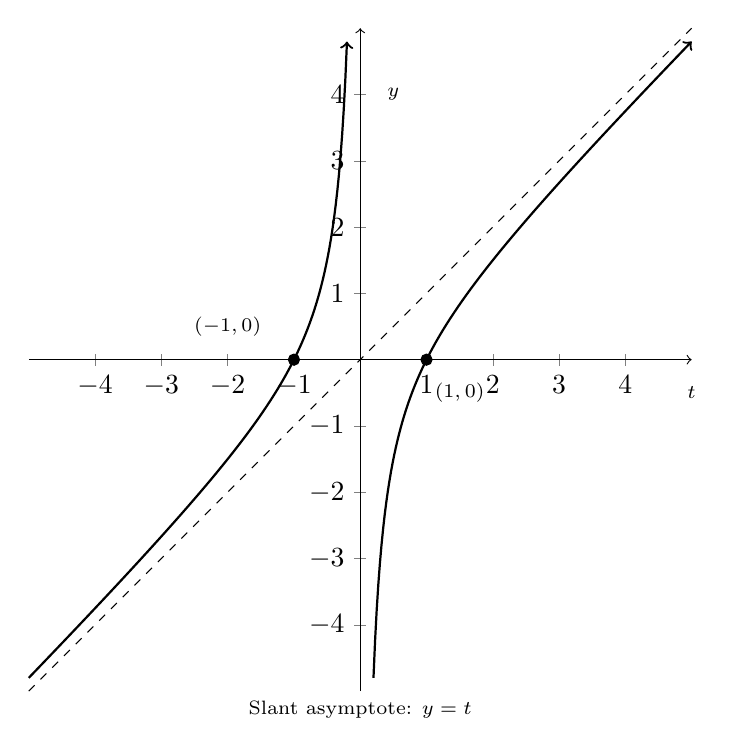
\begin{tikzpicture}
  \begin{axis}[
    axis lines=middle,
    xmin=-5, xmax=5,
    ymin=-5, ymax=5,
    xtick={-4,-3,-2,-1,1,2,3,4},
    xticklabels={$-4$,$-3$,$-2$,$-1$,$1$,$2$,$3$,$4$},
    ytick={-4,-3,-2,-1,1,2,3,4},
    yticklabels={$-4$,$-3$,$-2$,$-1$,$1$,$2$,$3$,$4$},
    axis line style={->},
    width=10cm, height=10cm,
    clip=false
  ]
    % Axis labels
    \node at (axis cs:5,-0.5) {\scriptsize $t$};
    \node at (axis cs:0.5,4) {\scriptsize $y$};

    % Slant asymptote y = t
    \addplot[dashed, domain=-5:5] {x};

    % Function pieces (avoiding asymptote at x=0)
    \addplot[domain=-5:-0.2, samples=200, thick, ->] {x - 1/x};
    \addplot[domain=0.2:5, samples=200, thick, ->] {x - 1/x};

    % Points
    \addplot[only marks, mark=*] coordinates {(-1,0) (1,0)};
    \node at (axis cs:-2,0.5) {\scriptsize $(-1,0)$};
    \node at (axis cs:1.5,-0.5) {\scriptsize $(1,0)$};

    % Caption
    \node[below] at (rel axis cs:0.5,0) 
      {\scriptsize Slant asymptote: $y=t$};
  \end{axis}
\end{tikzpicture}

\begin{solution}
$g(t) =\dfrac{t^2-1}{t}$
\end{solution}

\end{problem}

\begin{problem}\label{rationalfromgraphlast}
Find a possible formula for the function whose graph is given.
$y = G(t)$

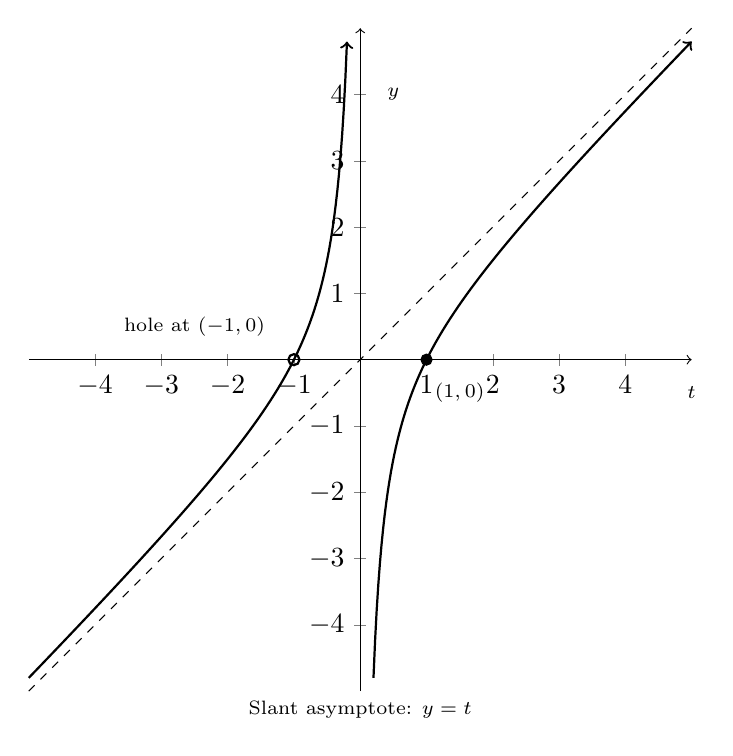
\begin{tikzpicture}
  \begin{axis}[
    axis lines=middle,
    xmin=-5, xmax=5,
    ymin=-5, ymax=5,
    xtick={-4,-3,-2,-1,1,2,3,4},
    xticklabels={$-4$,$-3$,$-2$,$-1$,$1$,$2$,$3$,$4$},
    ytick={-4,-3,-2,-1,1,2,3,4},
    yticklabels={$-4$,$-3$,$-2$,$-1$,$1$,$2$,$3$,$4$},
    axis line style={->},
    width=10cm, height=10cm,
    clip=false
  ]
    % Axis labels
    \node at (axis cs:5,-0.5) {\scriptsize $t$};
    \node at (axis cs:0.5,4) {\scriptsize $y$};

    % Slant asymptote y = t
    \addplot[dashed, domain=-5:5] {x};

    % Function pieces (avoiding discontinuity at x=0)
    \addplot[domain=-5:-0.2, samples=200, thick, ->] {x - 1/x};
    \addplot[domain=0.2:5, samples=200, thick, ->] {x - 1/x};

    % Open circle (hole) at (-1,0)
    \addplot[only marks, mark=o, mark size=2pt, thick] coordinates {(-1,0)};
    \node at (axis cs:-2.5,0.5) {\scriptsize hole at $(-1,0)$};

    % Solid point at (1,0)
    \addplot[only marks, mark=*] coordinates {(1,0)};
    \node at (axis cs:1.5,-0.5) {\scriptsize $(1,0)$};

    % Caption
    \node[below] at (rel axis cs:0.5,0) 
      {\scriptsize Slant asymptote: $y=t$};
  \end{axis}
\end{tikzpicture}

\begin{solution}
$G(t) = \dfrac{(t^2-1)(t+1)}{t(t+1)} = \dfrac{t^3+t^2-t-1}{t^2+t}$
\end{solution}

\end{problem}
 
\begin{problem}
Let $g(x) = \displaystyle \frac{x^{4} - 8x^{3} + 24x^{2} - 72x + 135}{x^{3} - 9x^{2} + 15x - 7}.\;$  With the help of your classmates:

\begin{itemize}

\item  find the $x$- and $y$- intercepts of the graph of $g$.

\item   find all of the asymptotes of the graph of $g$ and any holes in the graph, if they exist.

\item find the intervals on which the function is increasing, the intervals on which it is decreasing and the local maximums and minimums, if any exist.

\item sketch the graph of $g$, using more than one picture if necessary to show all of the important features of the graph.

\end{itemize}
\end{problem}

\begin{problem}\label{rationalneedcalcfirst}
Example \ref{carefulanalysisneeded} showed us that the six-step procedure cannot tell us everything of importance about the graph of a rational function and that sometimes there are things that are easy to miss.  Without Calculus, we may need to use graphing utilities to reveal the hidden behavior of rational functions.  Working with your classmates, use a graphing utility to examine the graphs the rational function given.  Compare and contrast their features.  Which features can the six-step process reveal and which features cannot be detected by it?   

$f(x) = \dfrac{1}{x^{2} + 1}$
\end{problem}

\begin{problem}
Example \ref{carefulanalysisneeded} showed us that the six-step procedure cannot tell us everything of importance about the graph of a rational function and that sometimes there are things that are easy to miss.  Without Calculus, we may need to use graphing utilities to reveal the hidden behavior of rational functions.  Working with your classmates, use a graphing utility to examine the graphs the rational function given.  Compare and contrast their features.  Which features can the six-step process reveal and which features cannot be detected by it?   

$f(x) = \dfrac{x}{x^{2} + 1}$ 
\end{problem}

\begin{problem}
Example \ref{carefulanalysisneeded} showed us that the six-step procedure cannot tell us everything of importance about the graph of a rational function and that sometimes there are things that are easy to miss.  Without Calculus, we may need to use graphing utilities to reveal the hidden behavior of rational functions.  Working with your classmates, use a graphing utility to examine the graphs the rational function given.  Compare and contrast their features.  Which features can the six-step process reveal and which features cannot be detected by it?  

$f(x) = \dfrac{x^{2}}{x^{2} + 1}$ 
\end{problem}

\begin{problem}\label{rationalneedcalclast}
Example \ref{carefulanalysisneeded} showed us that the six-step procedure cannot tell us everything of importance about the graph of a rational function and that sometimes there are things that are easy to miss.  Without Calculus, we may need to use graphing utilities to reveal the hidden behavior of rational functions.  Working with your classmates, use a graphing utility to examine the graphs the rational function given.  Compare and contrast their features.  Which features can the six-step process reveal and which features cannot be detected by it?   

$f(x) = \dfrac{x^{3}}{x^{2} + 1}$
\end{problem}

\end{document}
